\documentclass[11pt,UKenglish, a4paper]{article}
\usepackage[utf8]{inputenc}
%--fonts--
\usepackage[T1]{fontenc}
\usepackage[bitstream-charter]{mathdesign}

%--packages--
\usepackage[UKenglish]{babel}
\usepackage{csquotes,textcomp,varioref}

\usepackage{graphicx}
%--color--
\usepackage[dvipsnames]{xcolor}

%Setter inn pdfer
\usepackage[final]{pdfpages}

%-linespace--
\linespread{1.3}

%-Mer advansert liste--
\usepackage{enumitem}

%--hyperlinks-- include 
\usepackage[colorlinks=false, pdfborder={0 0 0}]{hyperref}

%--include subfiles-- 
\usepackage{subfiles}

%--fullpage--
%\usepackage{fullpage}

%--Uio-Front-Page--
%removed until it works \usepackage{ifikompendiumforside}

%--bibliography- -sortlocale=nb_No,
\usepackage[backend=biber, sortcites, defernumbers, style=numeric-comp, maxnames=2, natbib=true, backref, sorting=none, url=false]{biblatex}
%fjernet ifra style=authoryear-icomp
\addbibresource[datatype=bibtex]{Remote.bib}
%\addbibresource[datatype=bibtex]{Kilder.bib}

%farger jeg skal ha med
\definecolor{myY}{RGB}{241, 196, 15}
\definecolor{myB}{RGB}{52, 152, 219}
\definecolor{myG}{RGB}{46, 204, 113}
\definecolor{myLy}{RGB}{149, 165, 166}
\definecolor{myR}{rgb}{231, 76, 60}

%--Author and Title--
\author{Simon Lysne Hyenes}
\title{Participatory Sketching}

%--Latex Optimalization--
\tolerance = 5000
\hbadness = \tolerance
\pretolerance = 2000

%--Author and Title--
\author{Simon Lysne Hyenes}
\title{Participatory Sketching}

%--Starter--
\begin{document}
\section{Participatory Sketching}
Working with visualization and timelines framed the choice of tools and techniques in the early stages of the design process. A combination of participatory sketching and interviews was chosen. Participatory sketching is not a specific technique but a simplified process of problem setting, idea formulation and discussion. The term participatory signifying that the act of sketching is done by the participants with assistance from the faciliators. There are myriads of options for conducting such an exercise and all the details have to be explored and tested for the specific group, task and issue at hand. 

\subsection{Sketching and design}
Sketching is a drawing with a lack of details or lacking a complete finished character. There are many forms of sketching, the method I discuss here is drawing with ordinary utensils such as pen, pencil on paper. Stolterman refers to Kolko, Buxton and Morridge \cite[p.61]{Stolterman????Nature} as examples of designers that consider sketching at the core of the design practice.  
Fällman describes sketching as design thinking---sketches are ``an reflection of the guiding image''\cite[p.230]{Fallman2003DesignOriented}. Buxton, Fällman and others drawn on Schöns concepts of ``problem setting'' and ``problem solving''\cite[p.230]{Fallman2003DesignOriented}. Sketches enable a ``dialogue'' between problem setting and solving where design becomes a search for the whole---here sketches are intergral to the way designers think and work\cite[p.230]{Fallman2003DesignOriented}.

Fällman\cite[p.230]{Fallman2003DesignOriented}, Wang et.al \cite[p.2]{Wang2012User}, Tholander et. al\cite[p.446]{Tholander2008Where} point to three purposes for sketching: 
\begin{enumerate}
\item{Structure thoughts and ideas}
\item{Communication with oneself}
\item{Communcation with others}
\end{enumerate}

\subsection{Participatory Sketching}
Participatory sketching is one of the most open-ended forms of ``making'' techniques within participatory design. 
The core idea is that the participants sketch a prototype, solution, future vision or idea. At the most basic level it raises the engagement of the participants from observing to making. Once they are making this allows for several benefical things to take place. The participants become invested in an idea relating to your project. They articulate by their own means abstract ideas, side-stepping issues of definition power (sitat?) of technical language and jargon. If properly invested participants may engage freely and take greater care to describe and formulate their ideas to the group. The latter allow the participants to draw upon each others ideas and elaborate their ideas even further.
\subsubsection*{Making}
In participatory design tools and techniques are often judged on their ability to enable making, telling and enacting\cite[husker ikke hvem, fiks kilde.]{Bannon2012Design}. 

\subsubsection*{Why sketching}
Mitchell and Nørgaard point to Buxtons use of the term sketching. Here the material and results are less important than their ability to be ``rapidly made, provoke new questions, and provide the possibility to explore design assumptions quickly and at a low cost''\cite[p.2]{Mitchell2011Using}. 
Mitchell and Nørgaard point to benefits and weaknesses for participatory design projects. First sketches serves as entrypoints to discussion about design matters. Secondly they allow for a new and different way of thinking for participants. Wang et. al found that sketches during user requirement gathering could help to ``tangibilizing communication; (2) contextualizing design concepts; and (3) unveiling underlying thoughts''\cite[p.9]{Wang2012User}. 

Their main weakness is in the raised need for facilitation and preparation. Other weaknesses depend upon the group dynamics, facilitator skills and the visualization possibilities for the project and the group. 

\subsubsection*{What do sketches prototype}
Houde and Hill describe how prototypes of interactive systems are often focused on certain properties. In the ``formative stages''\cite[p.1]{Houde1997What} the purpose of the prototype should be considered carefully. The applicability of sketching depends upon several factors, the purpose and goals depend on what the desired artifacts should be used for.

\begin{figure}[HoudeHillPrototypes]
    \centering
	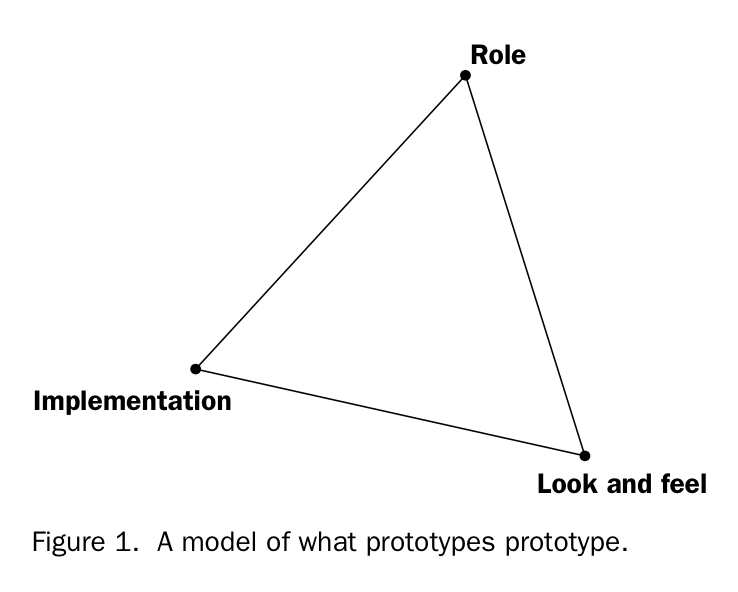
\includegraphics[width=0.5\linewidth]{Images/HoudeHillPrototypes}
    \caption{A model of what prototypes prototype\cite[p.3]{Houde1997What}}
    \label{fig:1}
\end{figure}

The sketches produced in workshops primarily display properties relating to ``role'' and to some degree to ``look and feel''. Participatory sketching can be used for several prototyping purposes. Depending upon the fidelity and clarity of the project the sketches themselves may not be regarded as specifically useful for the continued project. Instead the main benefit is their combined ability to generate useful and engaging participation during and beyond the end of the exercise. In this regard the sketches may not be considered prototypes but instead as boundary objects or design artifacts. As artifacts the sketches should be considered on different terms than they would have been as prototypes. 

\subsubsection*{Sketching, prototyping and participatory methods}
Fällman points to that within HCI and interaction design sketching is often subsumed under the umbrella term ``prototyping''\cite[p.230]{Fallman2003DesignOriented}. This is due to the limited ability to describe and present HCI concerns such as interactivity, temporality, tangibility etc\dots. Drawing upon Houde and Hill\cite[p.]{Houde1997What} Fällman claims that highlighting material properties and fidelity of the prototype may obscure the meaningful ``dialogue''\cite[p.230]{Fallman2003DesignOriented}. There are many tools and techniques within HCI-practice that build upon sketching. For instance storyboarding, collages..(mer her). 

In participatory design the choice of methods, tool and techniques is connected to their ability to...(hvordan velger man metoder i pd).
noe
\printbibliography
\end{document}
